\PassOptionsToPackage{unicode,pdftex}{hyperref}
\PassOptionsToPackage{hyphens}{url}
\documentclass[
]{article}
\usepackage[top=2.5cm,bottom=2.5cm,left=2.5cm,right=2.5cm]{geometry}
\usepackage{xcolor}
\setcounter{secnumdepth}{-\maxdimen}
\usepackage[T1]{fontenc}
\usepackage[utf8]{inputenc}
\usepackage{textcomp} % provide euro and other symbols
\usepackage{lmodern}
\IfFileExists{upquote.sty}{\usepackage{upquote}}{}
\IfFileExists{microtype.sty}{% use microtype if available
  \usepackage[protrusion=true,expansion=true]{microtype}
  \UseMicrotypeSet[protrusion]{basicmath} % disable protrusion for tt fonts
}{}
\usepackage{parskip}
\usepackage{fancyvrb}
\newcommand{\VerbBar}{|}
\newcommand{\VERB}{\Verb[commandchars=\\\{\}]}
\DefineVerbatimEnvironment{Highlighting}{Verbatim}{commandchars=\\\{\}}
\newenvironment{Shaded}{}{}
\newcommand{\AlertTok}[1]{\textcolor[rgb]{1.00,0.00,0.00}{\textbf{#1}}}
\newcommand{\AnnotationTok}[1]{\textcolor[rgb]{0.38,0.63,0.69}{\textbf{\textit{#1}}}}
\newcommand{\AttributeTok}[1]{\textcolor[rgb]{0.49,0.56,0.16}{#1}}
\newcommand{\BaseNTok}[1]{\textcolor[rgb]{0.25,0.63,0.44}{#1}}
\newcommand{\BuiltInTok}[1]{\textcolor[rgb]{0.00,0.50,0.00}{#1}}
\newcommand{\CharTok}[1]{\textcolor[rgb]{0.25,0.44,0.63}{#1}}
\newcommand{\CommentTok}[1]{\textcolor[rgb]{0.38,0.63,0.69}{\textit{#1}}}
\newcommand{\CommentVarTok}[1]{\textcolor[rgb]{0.38,0.63,0.69}{\textbf{\textit{#1}}}}
\newcommand{\ConstantTok}[1]{\textcolor[rgb]{0.53,0.00,0.00}{#1}}
\newcommand{\ControlFlowTok}[1]{\textcolor[rgb]{0.00,0.44,0.13}{\textbf{#1}}}
\newcommand{\DataTypeTok}[1]{\textcolor[rgb]{0.56,0.13,0.00}{#1}}
\newcommand{\DecValTok}[1]{\textcolor[rgb]{0.25,0.63,0.44}{#1}}
\newcommand{\DocumentationTok}[1]{\textcolor[rgb]{0.73,0.13,0.13}{\textit{#1}}}
\newcommand{\ErrorTok}[1]{\textcolor[rgb]{1.00,0.00,0.00}{\textbf{#1}}}
\newcommand{\ExtensionTok}[1]{#1}
\newcommand{\FloatTok}[1]{\textcolor[rgb]{0.25,0.63,0.44}{#1}}
\newcommand{\FunctionTok}[1]{\textcolor[rgb]{0.02,0.16,0.49}{#1}}
\newcommand{\ImportTok}[1]{\textcolor[rgb]{0.00,0.50,0.00}{\textbf{#1}}}
\newcommand{\InformationTok}[1]{\textcolor[rgb]{0.38,0.63,0.69}{\textbf{\textit{#1}}}}
\newcommand{\KeywordTok}[1]{\textcolor[rgb]{0.00,0.44,0.13}{\textbf{#1}}}
\newcommand{\NormalTok}[1]{#1}
\newcommand{\OperatorTok}[1]{\textcolor[rgb]{0.40,0.40,0.40}{#1}}
\newcommand{\OtherTok}[1]{\textcolor[rgb]{0.00,0.44,0.13}{#1}}
\newcommand{\PreprocessorTok}[1]{\textcolor[rgb]{0.74,0.48,0.00}{#1}}
\newcommand{\RegionMarkerTok}[1]{#1}
\newcommand{\SpecialCharTok}[1]{\textcolor[rgb]{0.25,0.44,0.63}{#1}}
\newcommand{\SpecialStringTok}[1]{\textcolor[rgb]{0.73,0.40,0.53}{#1}}
\newcommand{\StringTok}[1]{\textcolor[rgb]{0.25,0.44,0.63}{#1}}
\newcommand{\VariableTok}[1]{\textcolor[rgb]{0.10,0.09,0.49}{#1}}
\newcommand{\VerbatimStringTok}[1]{\textcolor[rgb]{0.25,0.44,0.63}{#1}}
\newcommand{\WarningTok}[1]{\textcolor[rgb]{0.38,0.63,0.69}{\textbf{\textit{#1}}}}
\usepackage{longtable,booktabs,array}
\renewcommand{\arraystretch}{1.3}
\usepackage{calc} % for calculating minipage widths
\usepackage{etoolbox}
\makeatletter
\patchcmd\longtable{\par}{\if@noskipsec\mbox{}\fi\par}{}{}
\makeatother
\usepackage{float}
\usepackage{graphicx}
\makeatletter
\newsavebox\pandoc@box
\newcommand*\pandocbounded[1]{% scales image to fit in text height/width
  \sbox\pandoc@box{#1}%
  \Gscale@div\@tempa{\textheight}{\dimexpr\ht\pandoc@box+\dp\pandoc@box\relax}%
  \Gscale@div\@tempb{\linewidth}{\wd\pandoc@box}%
  \ifdim\@tempb\p@<\@tempa\p@\let\@tempa\@tempb\fi% select the smaller of both
  \ifdim\@tempa\p@<\p@\scalebox{\@tempa}{\usebox\pandoc@box}%
  \else\usebox{\pandoc@box}%
  \fi%
}
\def\fps@figure{H}
\makeatother
\usepackage[english,polish]{babel}
\setlength{\emergencystretch}{3em} % prevent overfull lines
\providecommand{\tightlist}{%
\setlength{\itemsep}{0pt}\setlength{\parskip}{0pt}}
\usepackage{hyperref}
\usepackage{bookmark}
\IfFileExists{xurl.sty}{\usepackage{xurl}}{} % add URL line breaks if available
\urlstyle{same}
\hypersetup{
  pdflang={pl},
  hidelinks,
pdfcreator={LaTeX via pandoc}}

\author{}
\date{}

\begin{document}

\section{Analiza Danych Formuły 1: Jak technika zmieniała wyścigi przez ponad 70 lat}\label{analiza-danych-formuux142y-1-jak-technika-zmieniaux142a-wyux15bcigi-przez-ponad-70-lat}

\textbf{Przedmiot:} Analiza danych w języku Python (biblioteka pandas)
\textbf{Skład sekcji (zespołu):} Igor Barcik, Łukasz Domagała
\textbf{Kierunek:} Informatyka
\textbf{Rok:} 2026

\begin{center}\rule{0.5\linewidth}{0.5pt}
\end{center}

\tableofcontents

\begin{center}\rule{0.5\linewidth}{0.5pt}
\end{center}

\subsection{1. Co badamy i dlaczego}\label{co-badamy-i-dlaczego}

W Formule 1 wynik na torze zależy nie tylko od kierowcy, ale przede wszystkim od techniki --- od tego,
jak dobry jest bolid. Co kilka lat zmieniają się przepisy (np. inny rodzaj silnika), a inżynierowie
budują coraz lepsze auta. Każda taka zmiana zostawia ślad w liczbach: w czasach okrążeń, w liczbie
zwycięstw, w tym ile aut dojeżdża do mety.

\textbf{Cel projektu:} sprawdzić na liczbach, jak postęp techniczny zmieniał wyścigi przez 77 sezonów
(lata 1950--2026). Patrzymy na trzy rzeczy: jak szybkie były auta, jak bardzo były awaryjne i jak
wyrównana była walka między zespołami.

Pytania, na które szukamy odpowiedzi:

\begin{itemize}
    \tightlist
  \item
    \textbf{Czy auta dziś rzadziej się psują niż kiedyś?} Czyli: czy dojechanie do mety stało się normą?
  \item
    \textbf{Czy auta z roku na rok jeżdżą coraz szybciej?} Czy może czasem zwalniają, bo nowe przepisy
    „cofają'' rozwój?
  \item
    \textbf{Czy widać, że pełny bak paliwa spowalnia auto?} I czy widać w danych zakaz tankowania w czasie
    wyścigu (wprowadzony w 2010 roku)?
  \item
    \textbf{Czy zawsze wygrywają te same 2--3 zespoły, czy walka bywa bardziej wyrównana?}
  \item
    \textbf{Czy liczby pokazujące „talent'' kierowcy są uczciwe?} Czy łatwo nimi zmanipulować wynik?
\end{itemize}

Projekt jest \textbf{opisowy} --- to znaczy, że opisujemy i tłumaczymy, co się działo, ale nie przewidujemy
przyszłości. Ważne: przy każdej liczbie mówimy też, kiedy może ona mylić. Pokazanie słabości danej
miary jest tak samo cenne jak sama liczba.

\begin{center}\rule{0.5\linewidth}{0.5pt}
\end{center}

\subsection{2. Skąd dane i co zawierają}\label{skux105d-dane-i-co-zawierajux105}

\subsubsection{2.1. Skąd wzięliśmy dane}\label{skux105d-wziux119liux15bmy-dane}

Dane pochodzą z darmowej, publicznej bazy wyników F1 (projekt \textbf{Ergast}, udostępniony na platformie
\textbf{Kaggle}). To zwykłe pliki \textbf{CSV} (tabele z danymi, jak w Excelu).

Pliki wczytujemy do \textbf{DuckDB}. DuckDB to mała baza danych, która rozumie język \textbf{SQL} (język do
zadawania pytań danym, np. „pokaż wszystkie wyścigi z 2020 roku''). Działa szybko i nie wymaga osobnego
serwera --- uruchamia się od razu w programie. Dzięki temu możemy zadawać pytania nawet do bardzo dużych
tabel (setki tysięcy wierszy) i od razu dostawać wynik w Pythonie.

\begin{Shaded}
  \begin{Highlighting}[]
    \CommentTok{\# Pobierz pliki CSV z Kaggle i wczytaj każdy jako osobną tabelę w bazie}
    \NormalTok{race\_data }\OperatorTok{=}\NormalTok{ kagglehub.dataset\_download(}\StringTok{"jtrotman/formula{-}1{-}race{-}data"}\NormalTok{)}
    \NormalTok{conn }\OperatorTok{=}\NormalTok{ duckdb.}\ExtensionTok{connect}\NormalTok{(}\StringTok{"f1.db"}\NormalTok{)}
    \ControlFlowTok{for}\NormalTok{ f }\KeywordTok{in}\NormalTok{ glob.glob(}\SpecialStringTok{f"}\SpecialCharTok{\{}\NormalTok{race\_data}\SpecialCharTok{\}}\SpecialStringTok{/*.csv"}\NormalTok{):}
    \NormalTok{    name }\OperatorTok{=}\NormalTok{ os.path.splitext(os.path.basename(f))[}\DecValTok{0}\NormalTok{]}
    \NormalTok{    conn.execute(}\SpecialStringTok{f"CREATE OR REPLACE TABLE }\SpecialCharTok{\{}\NormalTok{name}\SpecialCharTok{\}}\SpecialStringTok{ AS SELECT * FROM read\_csv\_auto(\textquotesingle{}}\SpecialCharTok{\{}\NormalTok{f}\SpecialCharTok{\}}\SpecialStringTok{\textquotesingle{})"}\NormalTok{)}
  \end{Highlighting}
\end{Shaded}

\subsubsection{2.2. Jak duże są dane}\label{jak-duux17ce-sux105-dane}

\begin{longtable}[c]{@{}
    >{\raggedright\arraybackslash}p{(\linewidth - 2\tabcolsep) * \real{0.62}}
  >{\raggedleft\arraybackslash}p{(\linewidth - 2\tabcolsep) * \real{0.38}}@{}}
  \toprule\noalign{}
  Co & Ile \\
  \midrule\noalign{}
  \endhead
  \bottomrule\noalign{}
  \endlastfoot
  Zakres lat & \textbf{1950 -- 2026} \\
  Liczba sezonów & 77 \\
  Liczba wyścigów (Grand Prix) & 1 171 \\
  Liczba kierowców & 865 \\
  Liczba zespołów (konstruktorów) & 214 \\
  Liczba torów & 78 \\
  Liczba pojedynczych okrążeń (tabela \texttt{lap\_times}) & \textbf{871 076} \\
\end{longtable}

\begin{quote}
  \textbf{Ważne o latach:} nie każda analiza obejmuje pełne 1950--2026. Niektóre dane zaczęto zapisywać
  później --- np. czasy pojedynczych okrążeń istnieją dopiero od lat 80./90. Sezon 2026 jest \textbf{w trakcie}
  (jeszcze się nie skończył), więc ostatni punkt na wykresach trzeba czytać ostrożnie.
\end{quote}

\subsubsection{2.3. Najważniejsze tabele}\label{najwaux17cniejsze-tabele}

Tabela = arkusz z danymi. Każda ma swój temat. Łączymy je ze sobą po wspólnych numerach (tzw.
identyfikatorach, np. \texttt{raceId} = numer wyścigu).

\begin{longtable}[c]{@{}
    >{\raggedright\arraybackslash}p{(\linewidth - 4\tabcolsep) * \real{0.18}}
    >{\raggedleft\arraybackslash}p{(\linewidth - 4\tabcolsep) * \real{0.12}}
  >{\raggedright\arraybackslash}p{(\linewidth - 4\tabcolsep) * \real{0.70}}@{}}
  \toprule\noalign{}
  Tabela & Liczba wierszy & Co zawiera \\
  \midrule\noalign{}
  \endhead
  \bottomrule\noalign{}
  \endlastfoot
  \texttt{races} & 1 171 & Kalendarz wyścigów: rok, runda, tor, data \\
  \texttt{results} & 27 348 & Wyniki: zajęte miejsce, punkty, czy auto dojechało do mety \\
  \texttt{lap\_times} & 871 076 & Czas każdego pojedynczego okrążenia \\
  \texttt{qualifying} & 11 080 & Wyniki kwalifikacji (walka o miejsce startowe) \\
  \texttt{pit\_stops} & 22 249 & Postoje w boksie (zmiana opon itd.) \\
  \texttt{drivers} & 865 & Kierowcy: imię, nazwisko, narodowość, data urodzenia \\
  \texttt{constructors} & 214 & Zespoły: nazwa, narodowość \\
  \texttt{status} & 140 & Słownik powodów zakończenia (np. „dojechał'', „silnik'', „kolizja'') \\
  \texttt{circuits} & 78 & Tory: nazwa, kraj, położenie \\
\end{longtable}

\subsubsection{2.4. Czyszczenie danych przed analizą}\label{czyszczenie-danych-przed-analizux105}

Surowe dane nigdy nie są idealne. Zanim coś policzymy, trzeba je posprzątać:

\begin{itemize}
    \tightlist
  \item
    \textbf{Braki danych} --- gdy czegoś brakuje, w plikach jest znak \texttt{\textbackslash{}N}. Takie wiersze pomijamy lub
    oznaczamy jako „puste''.
  \item
    \textbf{Łączenie tabel} --- sklejamy tabele po wspólnych numerach (np. wynik + nazwa kierowcy + nazwa toru).
  \item
    \textbf{Czas w milisekundach} --- czasy okrążeń zamieniamy na milisekundy, żeby dało się je dodawać
    i porównywać.
  \item
    \textbf{Usuwanie dziwnych wartości (metoda IQR)} --- IQR to prosty sposób na wyrzucenie wartości skrajnych.
    Np. okrążenie podczas postoju w boksie jest bardzo wolne i zaburzyłoby wynik, więc je odrzucamy.
  \item
    \textbf{Czy auto dojechało do mety} --- z powodu zakończenia robimy prostą informację: „dojechał'' albo
    „nie dojechał''.
\end{itemize}

\begin{center}\rule{0.5\linewidth}{0.5pt}
\end{center}

\subsection{3. Analiza danych}\label{analiza-danych}

Zrobiliśmy sześć osobnych analiz. Każda działa tak samo: pytamy bazę o dane (SQL), liczymy w Pythonie
(\texttt{pandas}, \texttt{numpy}) i rysujemy wykres (\texttt{matplotlib}, \texttt{seaborn}). Gdzie trzeba, rysujemy też \textbf{linię
trendu} --- gładką krzywą, która pokazuje ogólny kierunek mimo wahań.

\subsubsection{3.1. Jak ciężar paliwa wpływa na czas okrążenia}\label{jak-ciux119ux17car-paliwa-wpux142ywa-na-czas-okrux105ux17cenia}

\textbf{Co robimy.} Bierzemy dwa tory, które najczęściej gościły wyścigi (Silverstone i Hungaroring).
Patrzymy, jak zmienia się czas okrążenia w trakcie jednego wyścigu. Dzielimy historię na dwa okresy:
\textbf{gdy wolno było tankować w czasie wyścigu (1994--2009)} i \textbf{gdy zakazano tankowania (od 2010)}.

\textbf{Wynik.} Im więcej paliwa się spali, tym auto jest lżejsze i szybsze --- czasy okrążeń maleją w trakcie
wyścigu. Efekt jest \textbf{mocniejszy po 2010 roku}, bo wtedy auta startują z paliwem na cały wyścig (są
cięższe na starcie). Ten sam wzór widać na \textbf{obu torach} --- czyli to naprawdę wina ciężaru paliwa,
a nie przypadek na jednym torze.

\pandocbounded{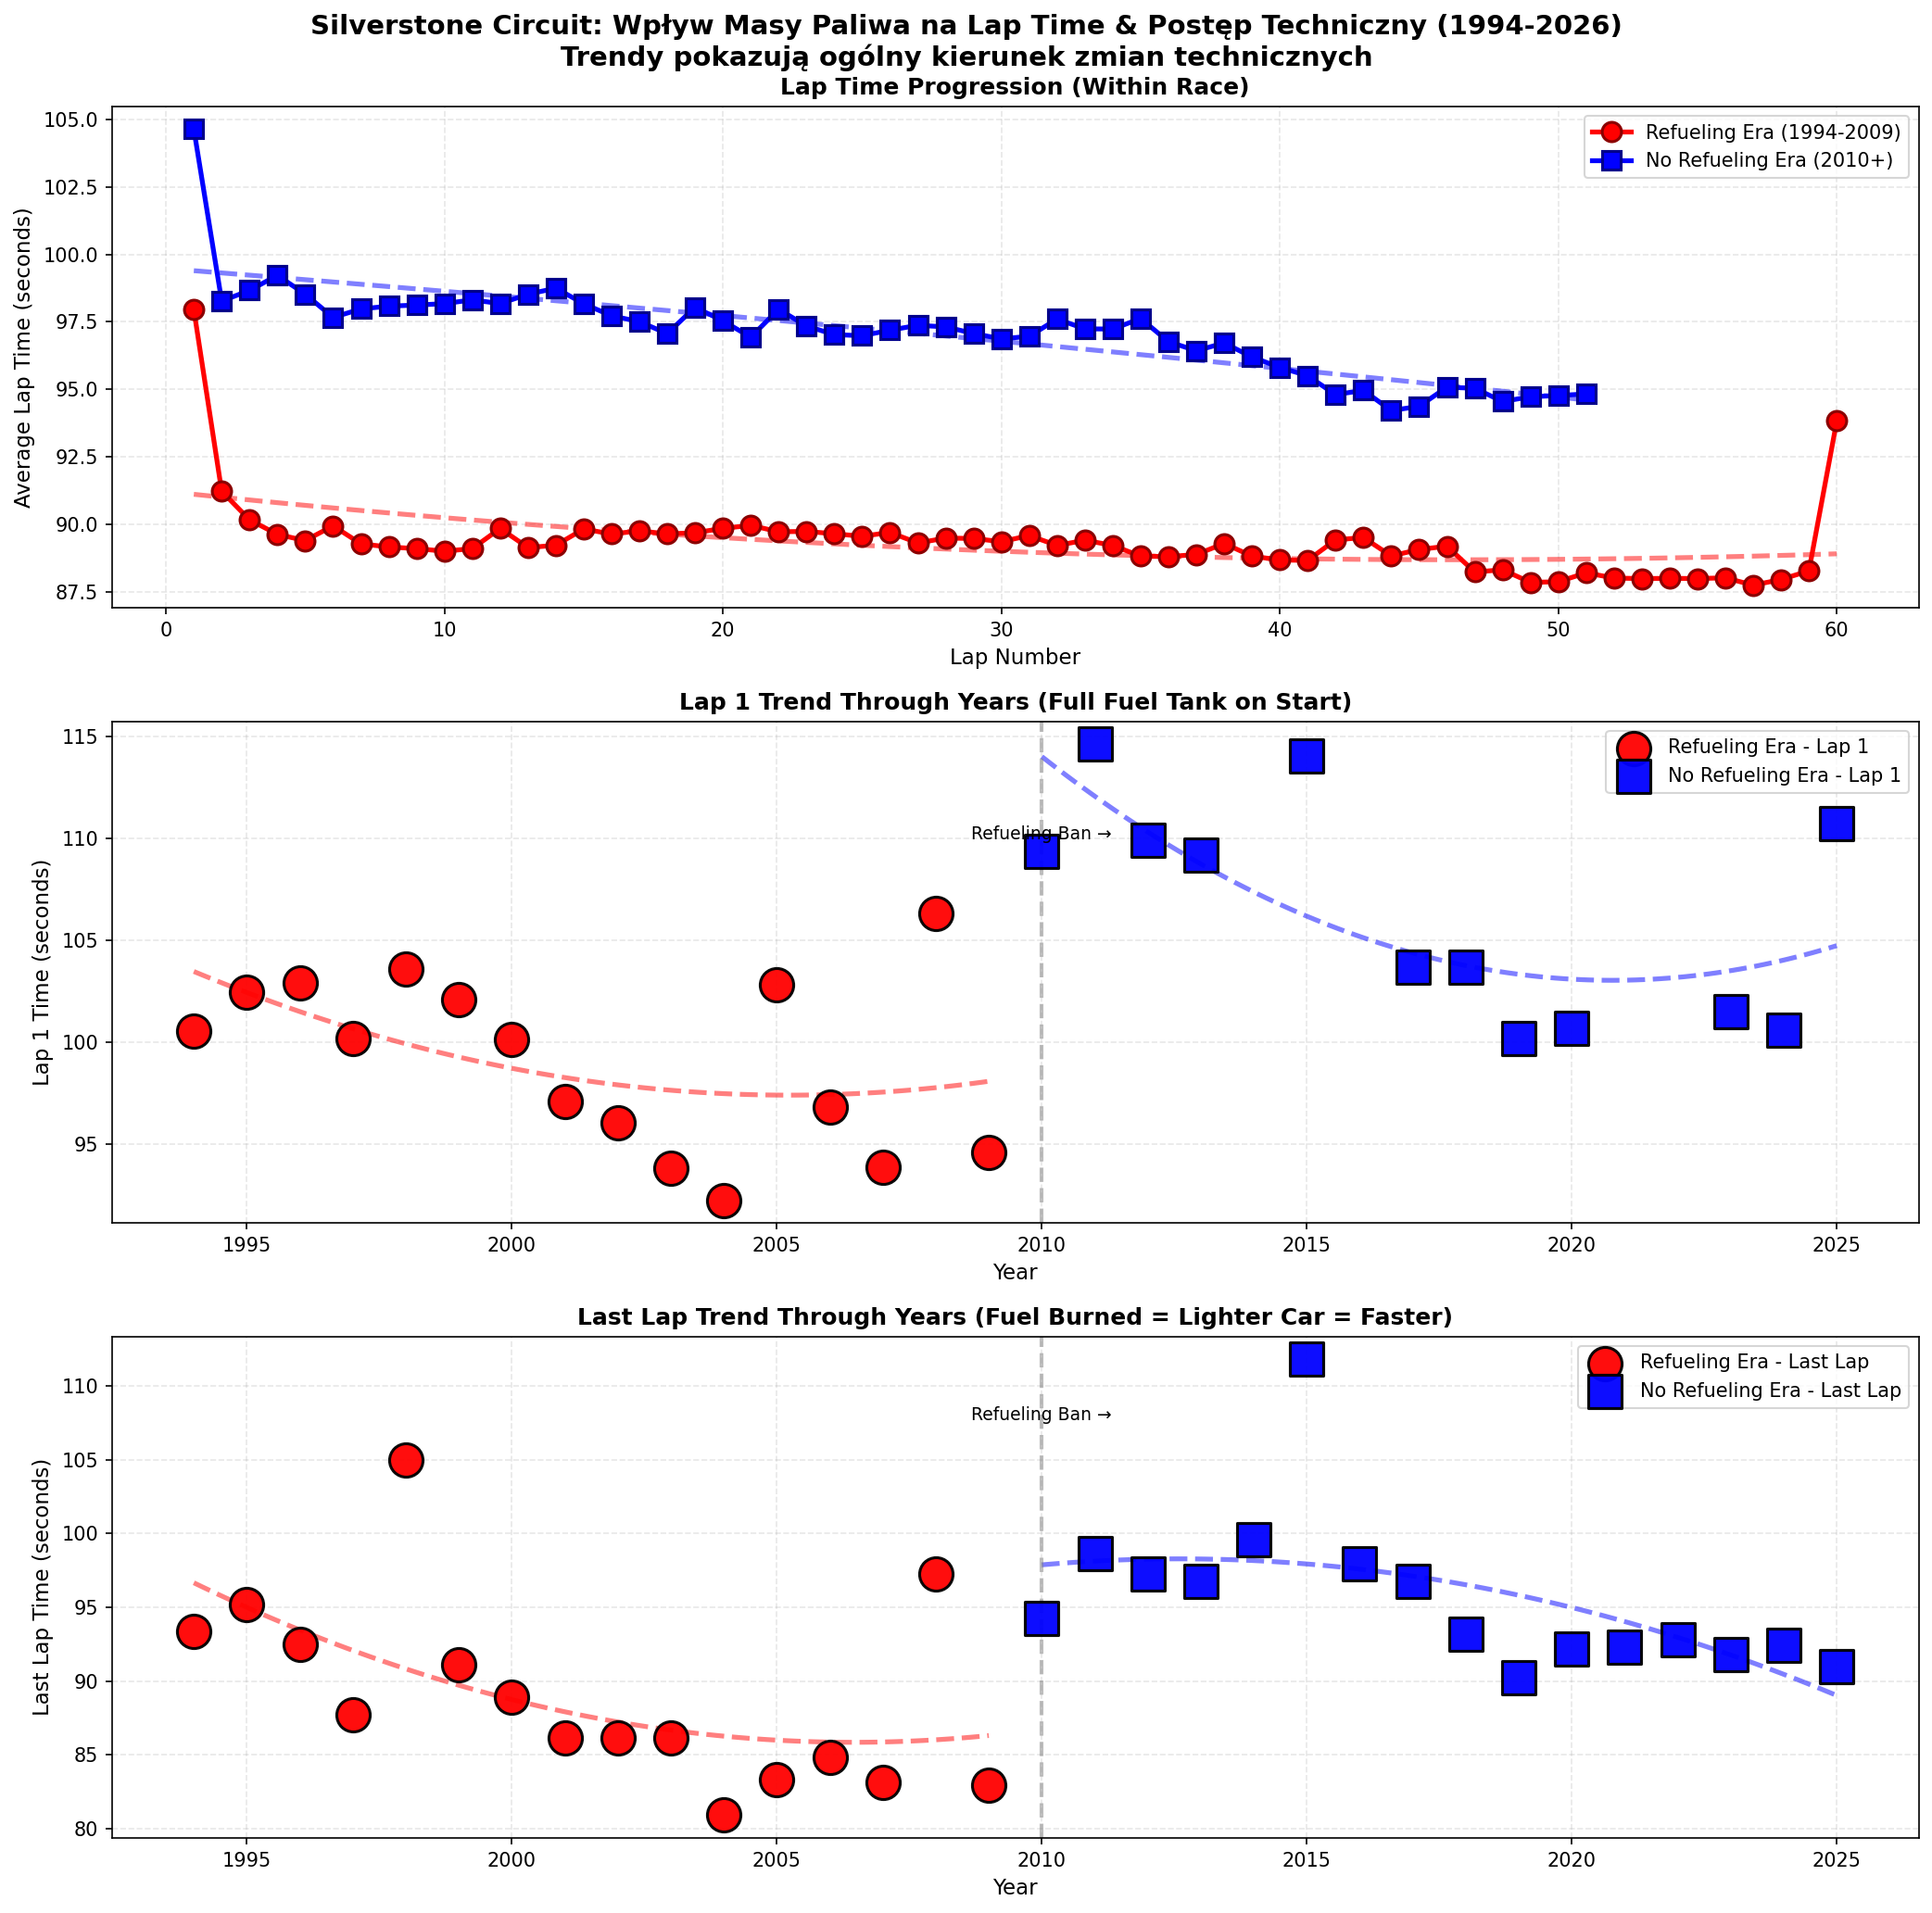
\includegraphics[keepaspectratio]{pres/F1Pandas/images/f1_fuel_impact_Silverstone_Circuit.png}}
\pandocbounded{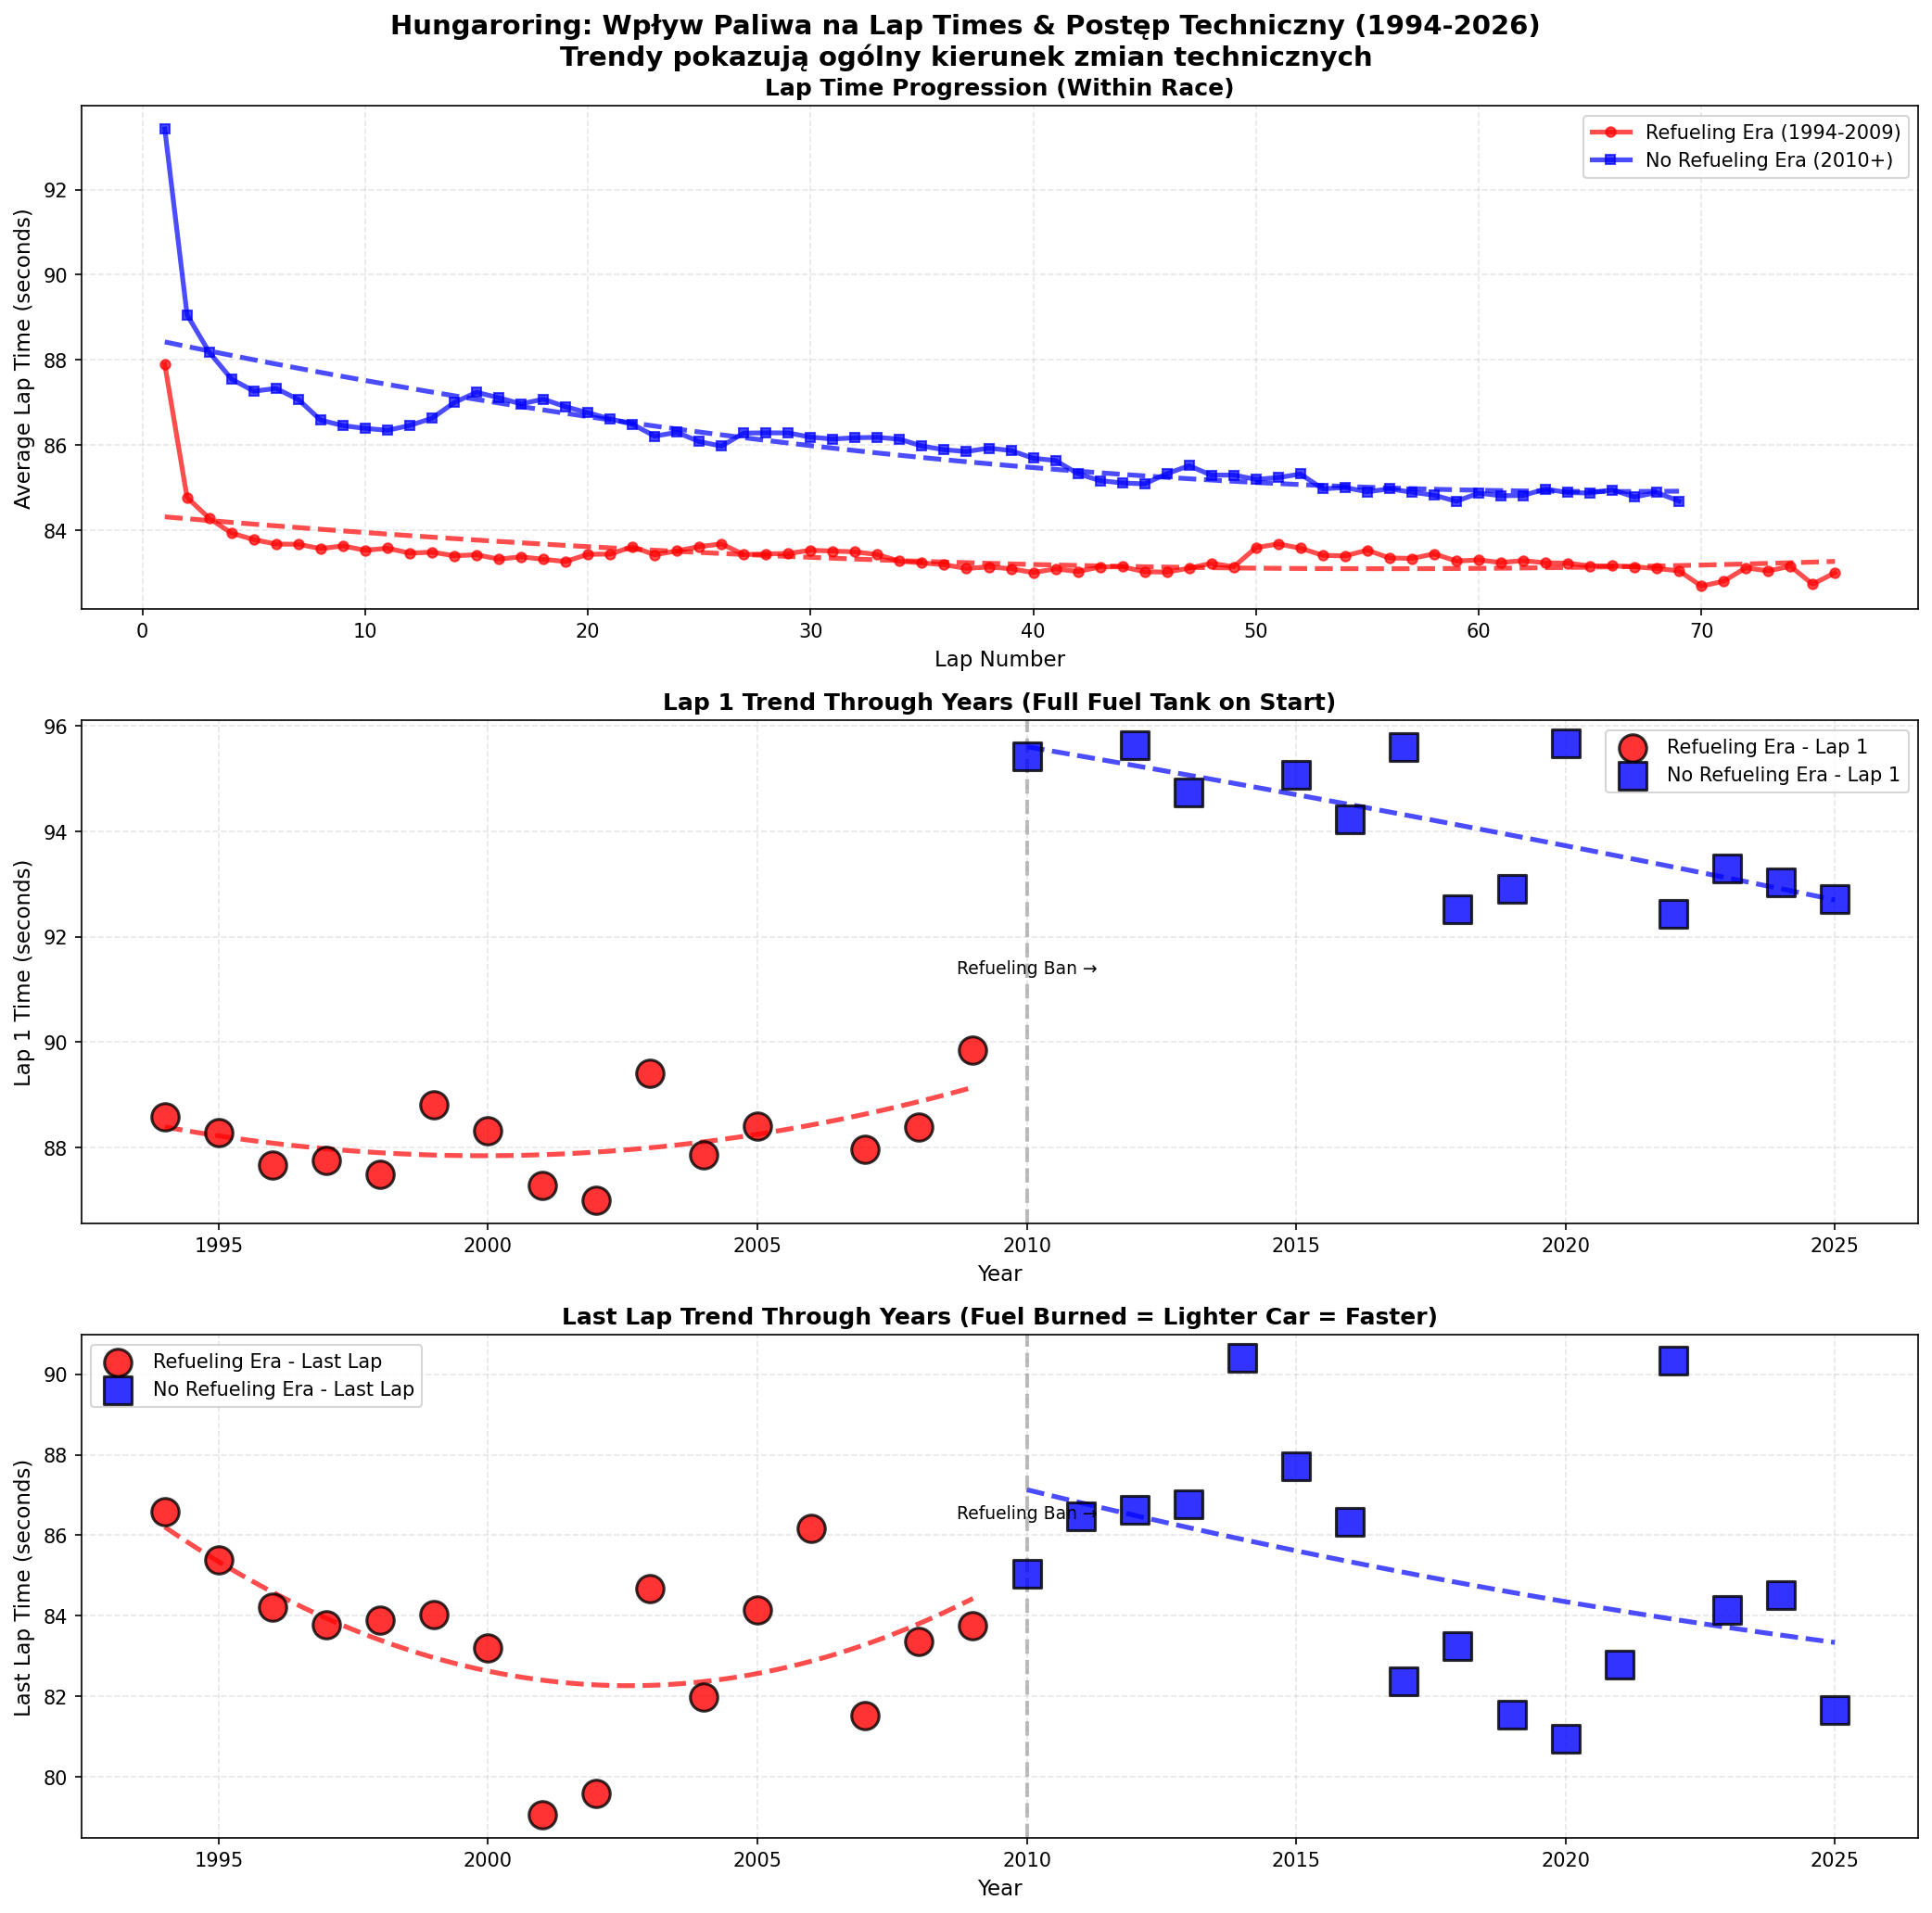
\includegraphics[keepaspectratio]{pres/F1Pandas/images/f1_fuel_impact_Hungaroring.png}}

\newpage
\subsubsection{3.2. Czy 3 najlepsze zespoły zgarniają wszystko}\label{czy-3-najlepsze-zespoux142y-zgarniajux105-wszystko}

\textbf{Co robimy.} Dla każdego sezonu liczymy, jaki \textbf{procent} wszystkich punktów zdobyły 3 najlepsze
zespoły. Liczymy procent (a nie samą liczbę punktów), bo zasady punktowania zmieniały się przez lata ---
procent jest sprawiedliwszy do porównań.

\textbf{Wynik.} Co sezon 3 czołowe zespoły biorą około 70--80\% punktów. Najbardziej dominowały w latach 50.
(aż \textasciitilde98\% w 1952). Potem walka się wyrównała (\textasciitilde51\% na początku lat 80.), a teraz znów dominacja rośnie
(np. Mercedes 2014--2020, później Red Bull). \textbf{Wniosek: dominacja kręci się w cyklach --- raz większa,
raz mniejsza.}

\begin{figure}
  \centering
  \pandocbounded{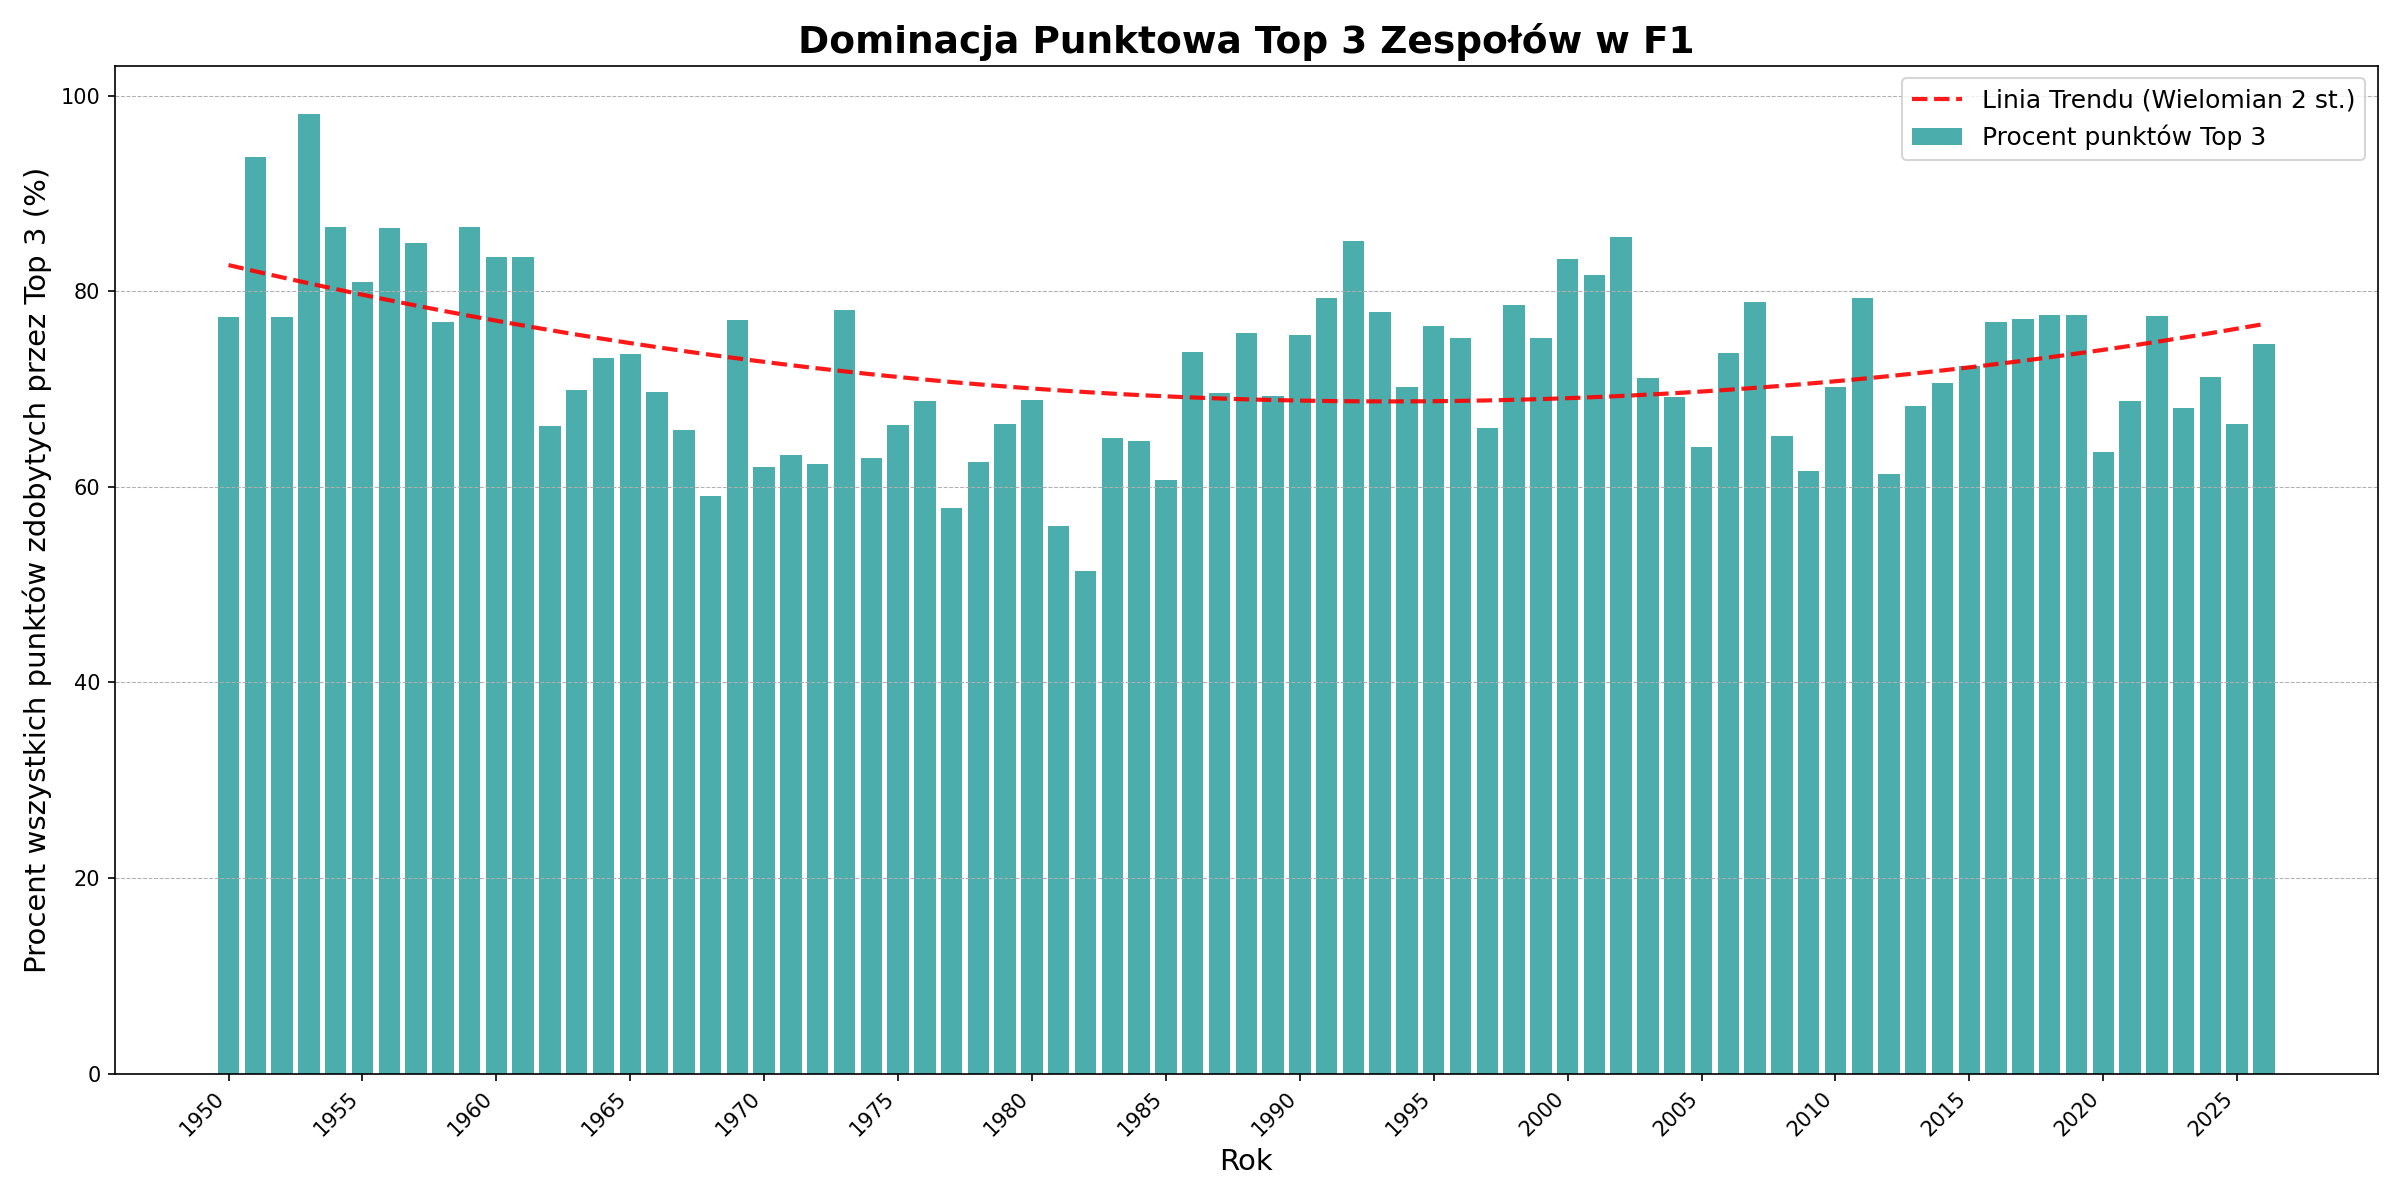
\includegraphics[keepaspectratio]{pres/F1Pandas/images/f1_top3_dominance_main.png}}
  \caption{Dominacja Top-3}
\end{figure}

\newpage
\subsubsection{3.3. Który zespół zdobywa najwięcej punktów na sezon}\label{ktuxf3ry-zespuxf3ux142-zdobywa-najwiux119cej-punktuxf3w-na-sezon}

\textbf{Co robimy.} Liczymy: suma wszystkich punktów zespołu ÷ liczba sezonów, w których jeździł
(minimum 3 sezony).

\textbf{Wynik --- uwaga, tu można się pomylić.} Najlepiej wypadają Mercedes (\textasciitilde440) i Red Bull (\textasciitilde370). Ale ta
miara \textbf{faworyzuje nowsze zespoły}, bo dziś za jeden wyścig rozdaje się dużo więcej punktów niż kiedyś
(dawniej zwycięstwo = \textasciitilde8 pkt, dziś = 25 pkt + punkty dla wielu kierowców). Dlatego stare, zasłużone
zespoły jak Ferrari (\textasciitilde150) wypadają gorzej, choć mają więcej tytułów. \textbf{Ta liczba mówi o tempie
zbierania punktów dziś --- a nie o tym, kto jest najlepszy w historii.}

\begin{figure}
  \centering
  \pandocbounded{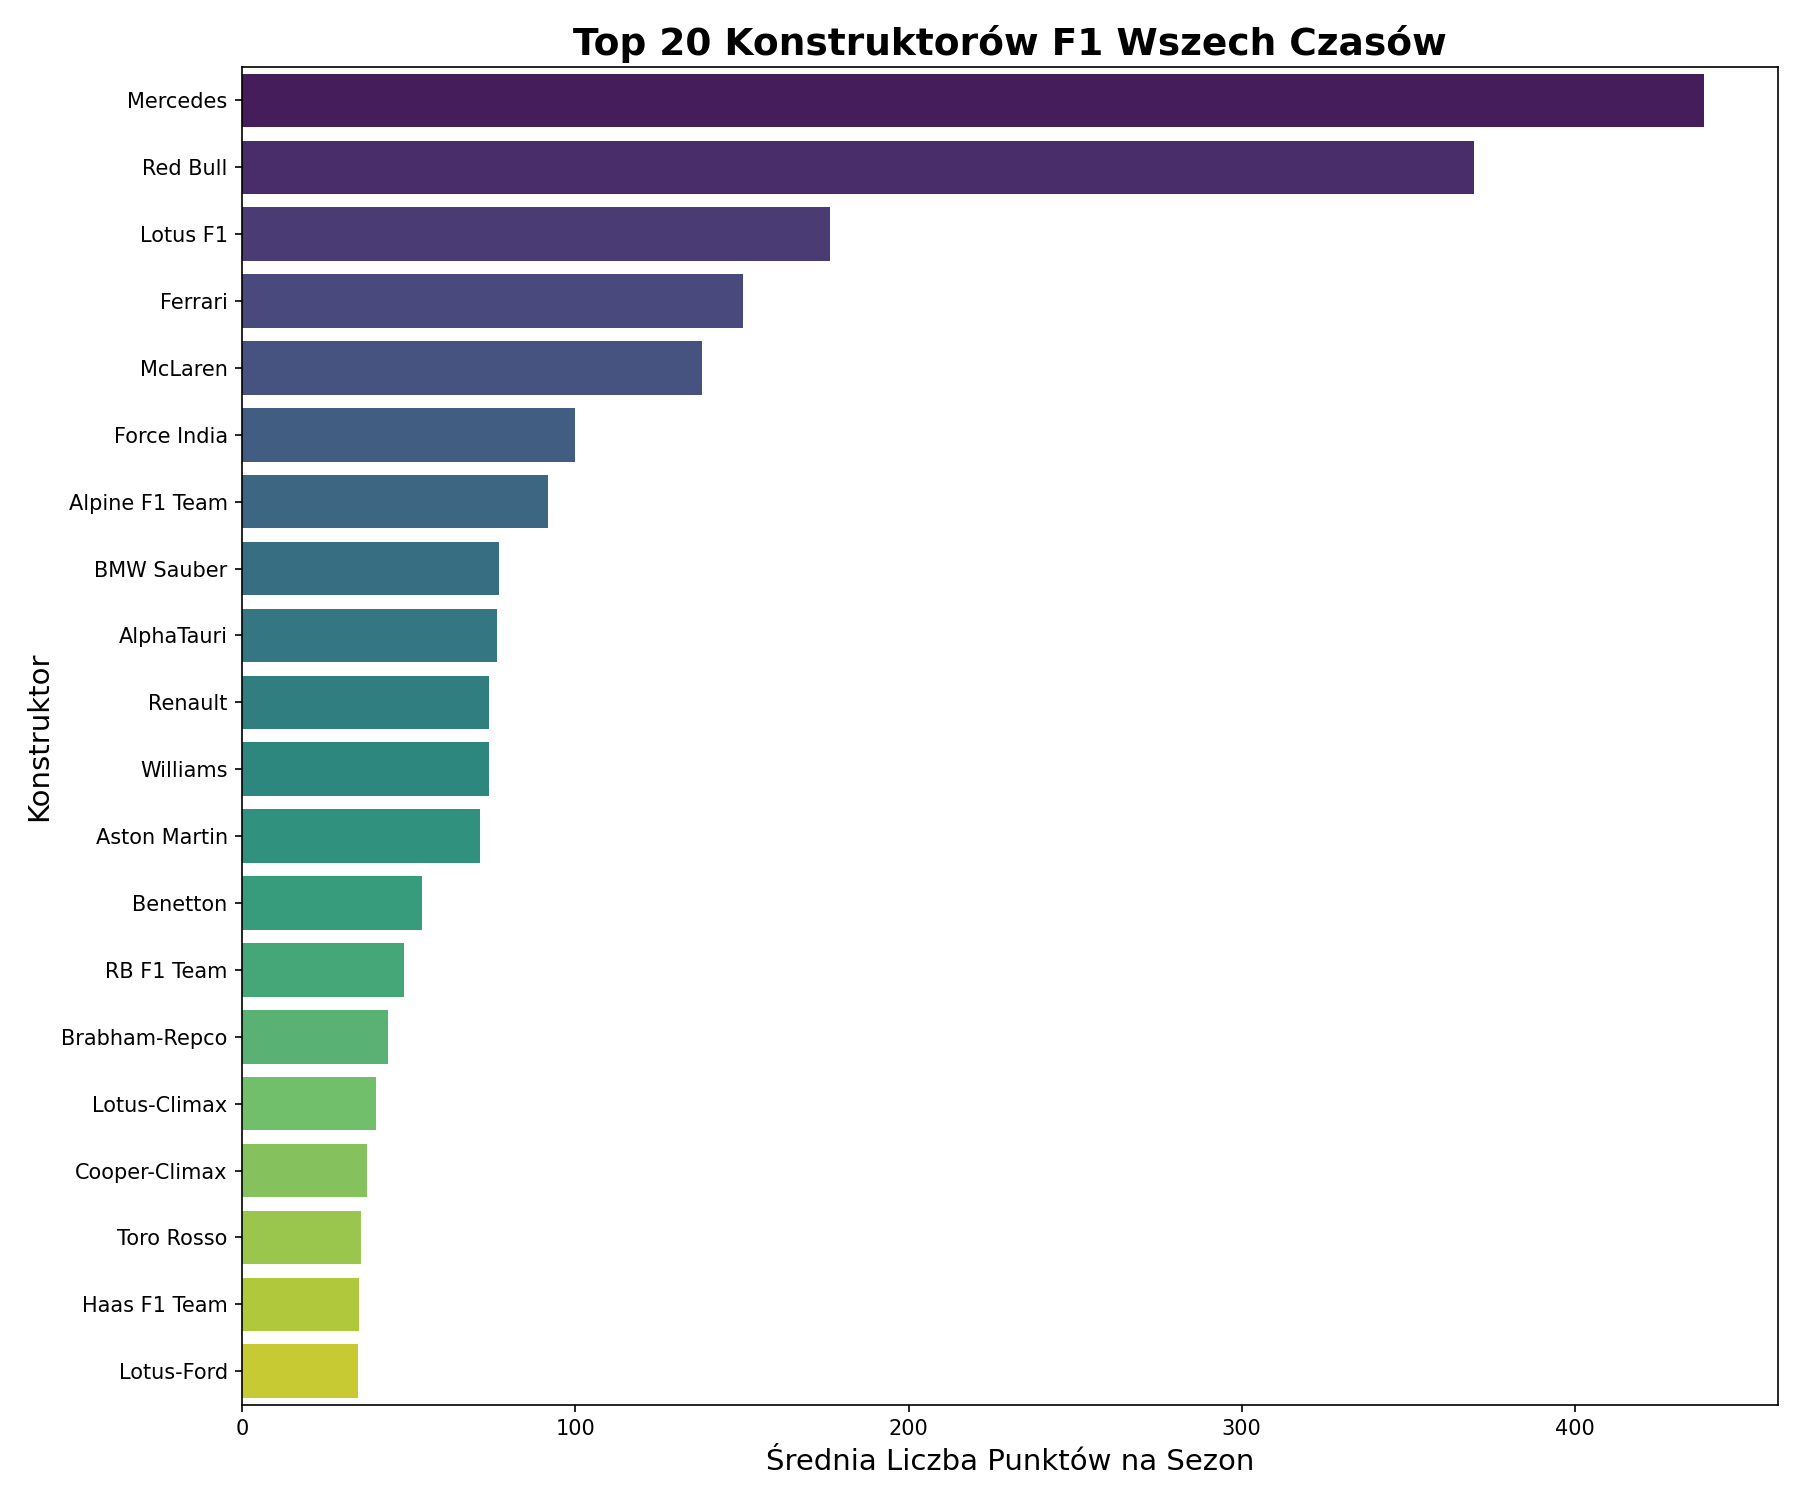
\includegraphics[keepaspectratio]{pres/F1Pandas/images/f1_top_constructors_by_points_per_season.png}}
  \caption{Konstruktorzy --- punkty na sezon}
\end{figure}

\newpage
\subsubsection{3.4. Czy auta dziś częściej dojeżdżają do mety (niezawodność)}\label{czy-auta-dziux15b-czux119ux15bciej-dojeux17cdux17cajux105-do-mety-niezawodnoux15bux107}

\textbf{Co robimy.} DNF to skrót od „nie ukończył wyścigu'' (ang. \emph{Did Not Finish}). Dla każdego sezonu
liczymy: ile aut nie dojechało ÷ ile wystartowało. To pokazuje, jak często auta się psuły.

\textbf{Wynik.} Kiedyś było bardzo źle --- pod koniec lat 60. nawet \textasciitilde47\% aut nie kończyło wyścigu (prawie
co drugie!). Dziś to tylko \textbf{10--15\%}. Dojechanie do mety zmieniło się z loterii w normę. \textbf{To
najmocniejszy dowód, że technika poszła do przodu.} Dwa zastrzeżenia: (1) do DNF liczą się też wypadki
i kolizje, nie tylko awarie; (2) mały wzrost na końcu wykresu to niedokończony sezon 2026, a nie realne
pogorszenie.

\begin{figure}
  \centering
  \pandocbounded{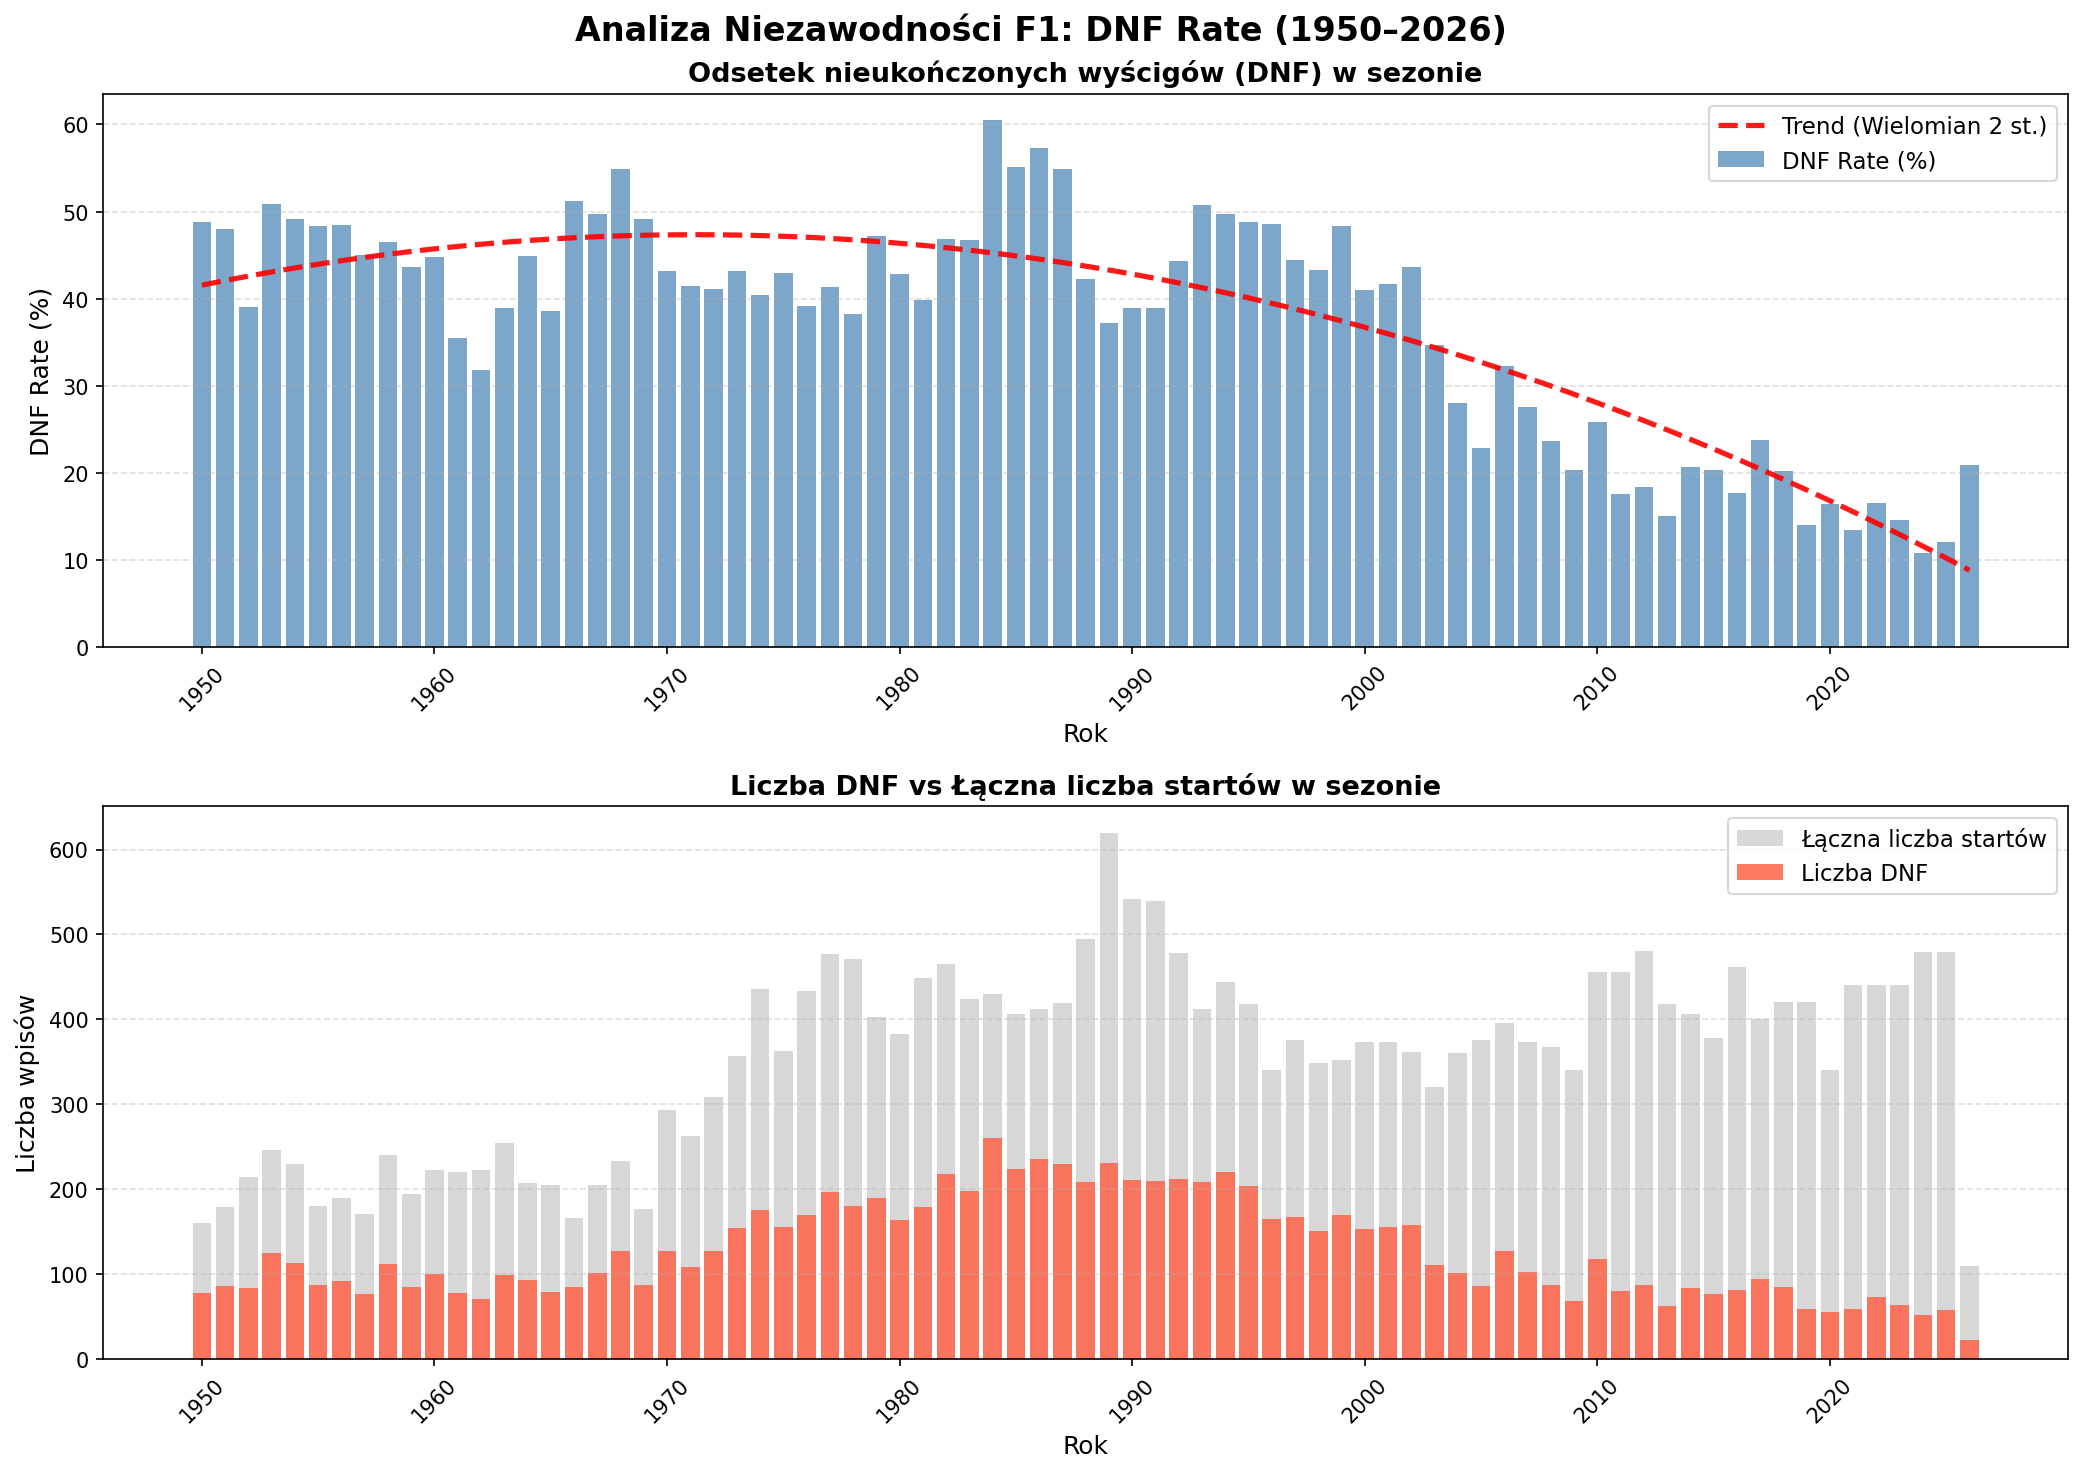
\includegraphics[keepaspectratio]{pres/F1Pandas/images/f1_dnf_reliability.png}}
  \caption{Trend DNF}
\end{figure}

\newpage
\subsubsection{3.5. Czy auta z roku na rok jeżdżą szybciej}\label{czy-auta-z-roku-na-rok-jeux17cdux17cux105-szybciej}

\textbf{Co robimy.} Z każdego wyścigu bierzemy jedno \textbf{najszybsze okrążenie}, a potem liczymy średnią dla
każdego roku. Sprawdzamy, czy czasy z roku na rok spadają (szybciej = lepiej).

\textbf{Wynik.} Auta \textbf{nie} robiły się szybsze równo z roku na rok. Najszybciej było na początku lat 2000.
Potem przyszły nowe przepisy w 2009 (mniej aerodynamiki) i 2014 (cięższe silniki hybrydowe) i auta
\textbf{zwolniły}, a dopiero później znów nadrabiały. Czyli postęp nie jest stały --- \textbf{co kilka lat przepisy
„resetują'' rozwój.} Uwaga: różne tory mają różną długość, więc patrzymy na ogólny trend, a nie na
pojedyncze lata.

\begin{figure}
  \centering
  \pandocbounded{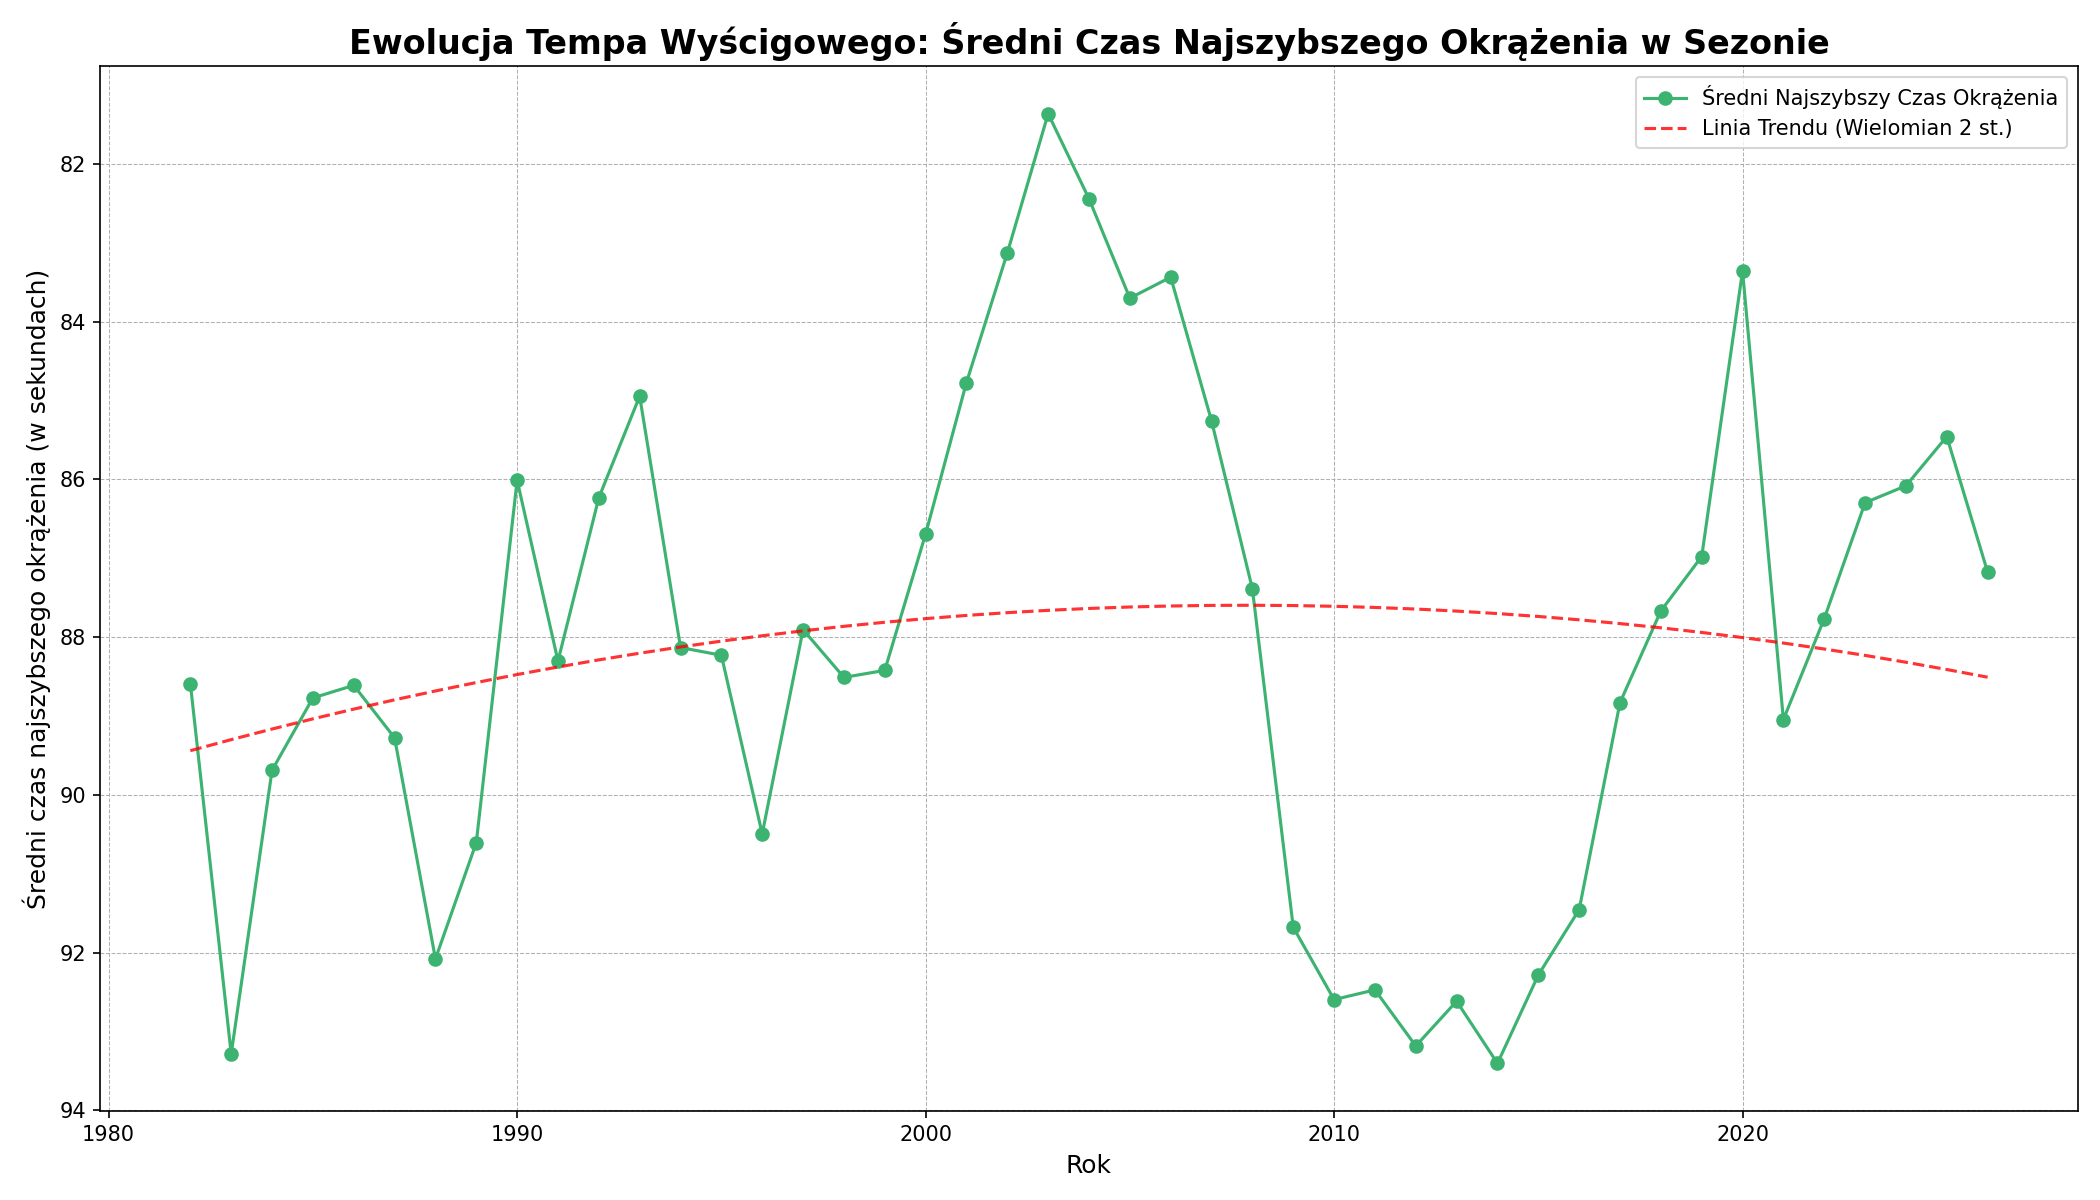
\includegraphics[keepaspectratio]{pres/F1Pandas/images/f1_moores_law_fastest_lap_from_laptimes.png}}
  \caption{Najszybsze okrążenia}
\end{figure}
\vfill
\subsubsection{3.6. Kto wygrywa z kolegą z tego samego zespołu}\label{kto-wygrywa-z-kolegux105-z-tego-samego-zespoux142u}

\textbf{Co robimy.} Dwóch kierowców z tego samego zespołu jeździ takim samym autem --- więc kto wyżej, ten
lepszy danego dnia. Liczymy, jaki procent takich „pojedynków'' wygrał każdy kierowca (bierzemy kierowców
z min. 50 wspólnymi wyścigami).

\textbf{Wynik.} Najwyżej jest Verstappen (\textasciitilde83\%), nisko Hamilton (\textasciitilde58\%). Ale ranking trzeba czytać ostrożnie:
łatwiej wygrywać, gdy ma się słabszego partnera, a trudniej, gdy partner jest mocny. Dodatkowo liczymy
tylko wyścigi, które obaj ukończyli (awarie pomijamy), i nie bierzemy pod uwagę, jak silny był rywal.
\textbf{Ta liczba mówi „jak często bił swojego kolegę'' --- a nie kto jest najlepszy w ogóle.}

\begin{figure}
  \centering
  \pandocbounded{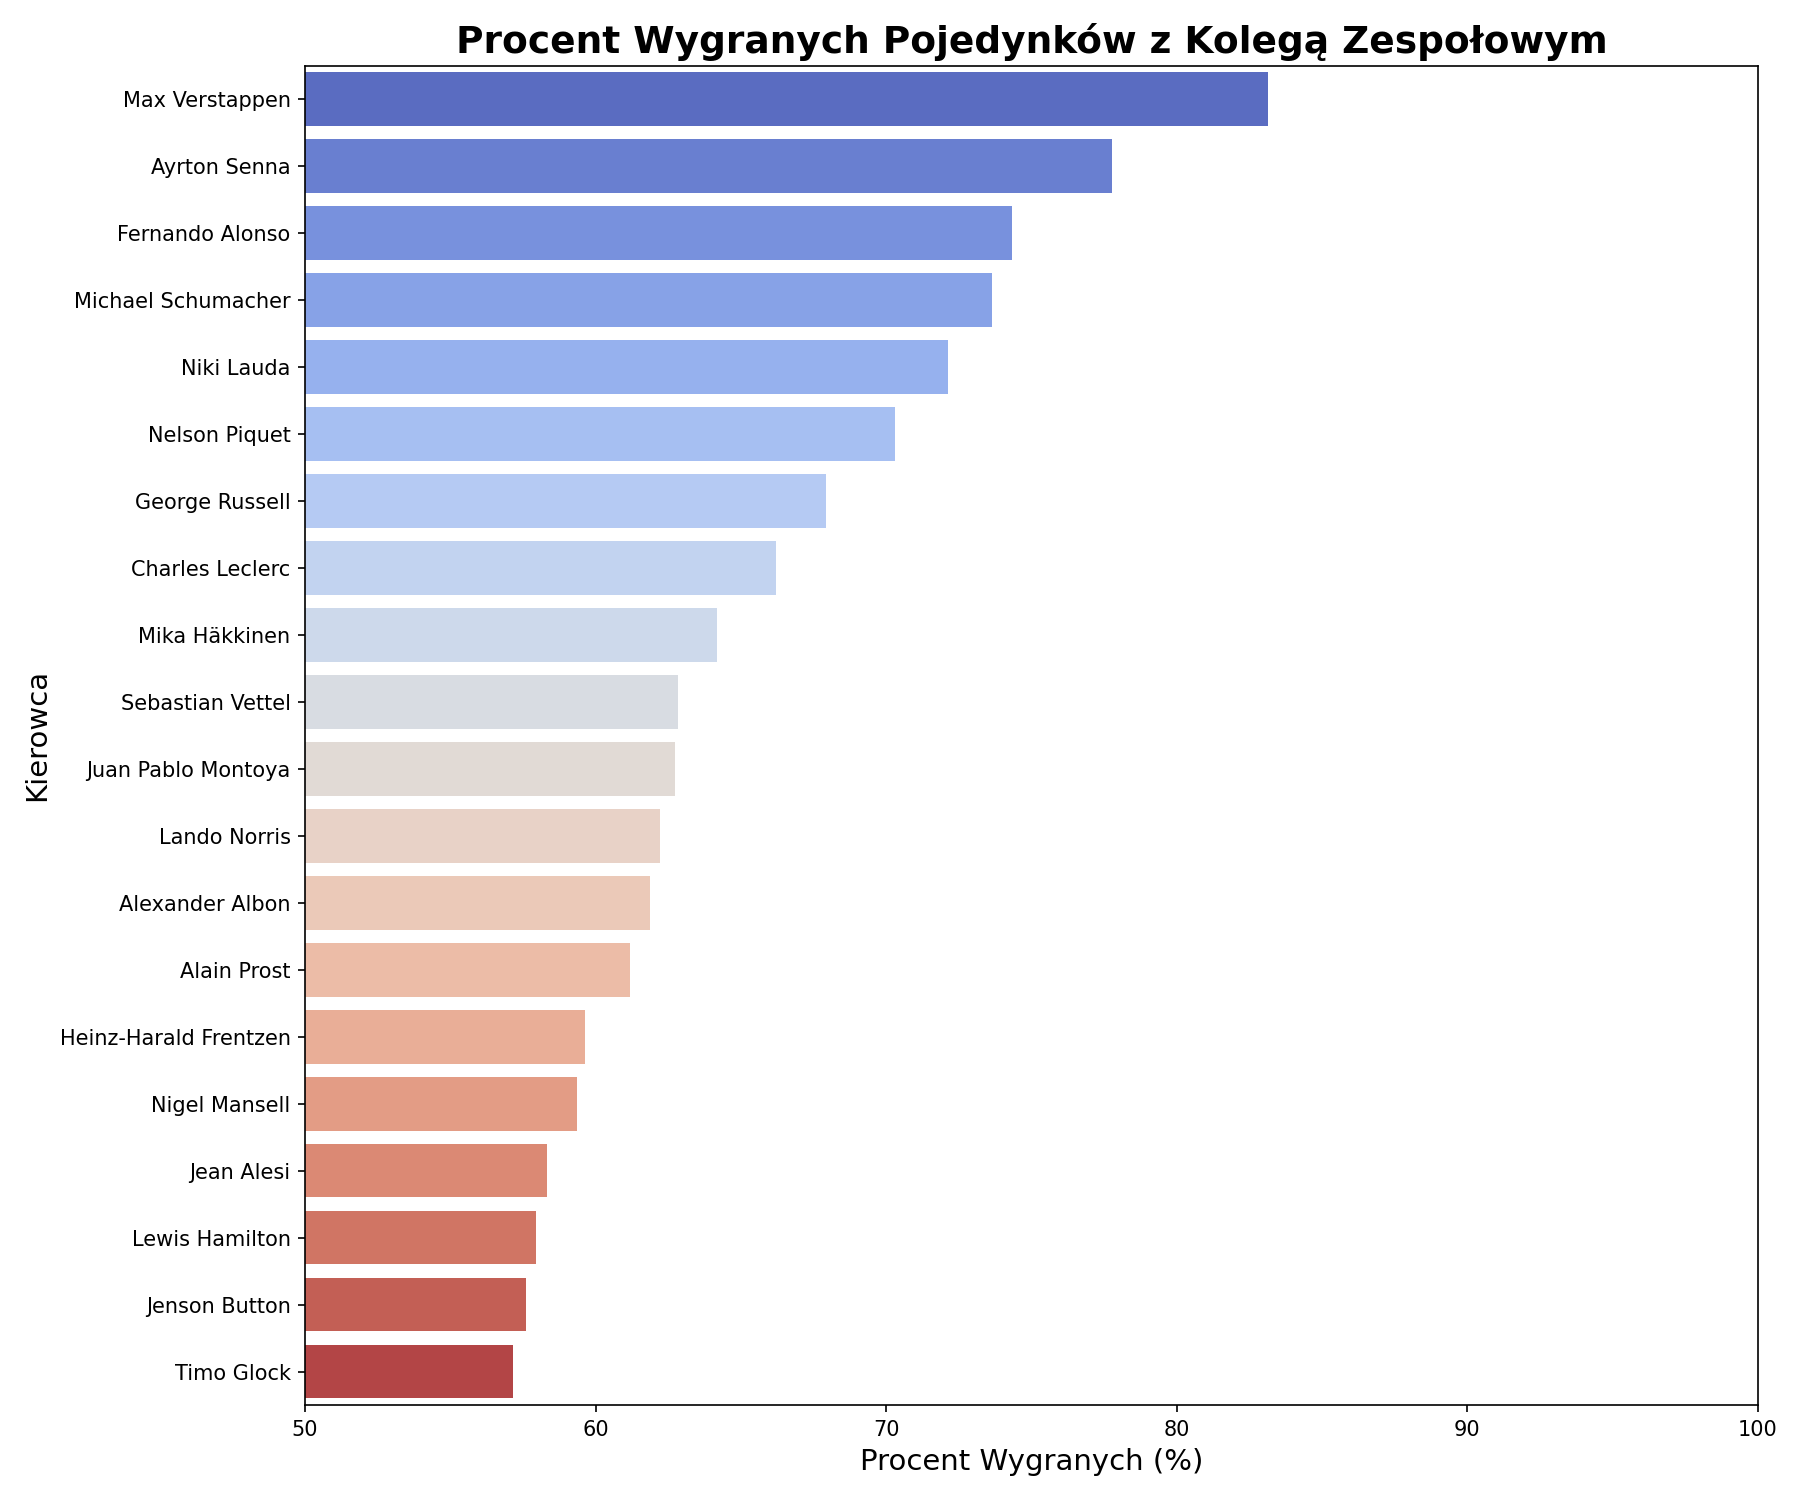
\includegraphics[keepaspectratio]{pres/F1Pandas/images/f1_teammate_duels.png}}
  \caption{Pojedynki w zespole}
\end{figure}

\newpage
\subsubsection{3.7. Wykres zbiorczy}\label{wykres-zbiorczy}

Najważniejsze wyniki (niezawodność, szybkość, dominacja, wpływ paliwa) zebraliśmy na jednym wspólnym
obrazku.

\begin{figure}
  \centering
  \pandocbounded{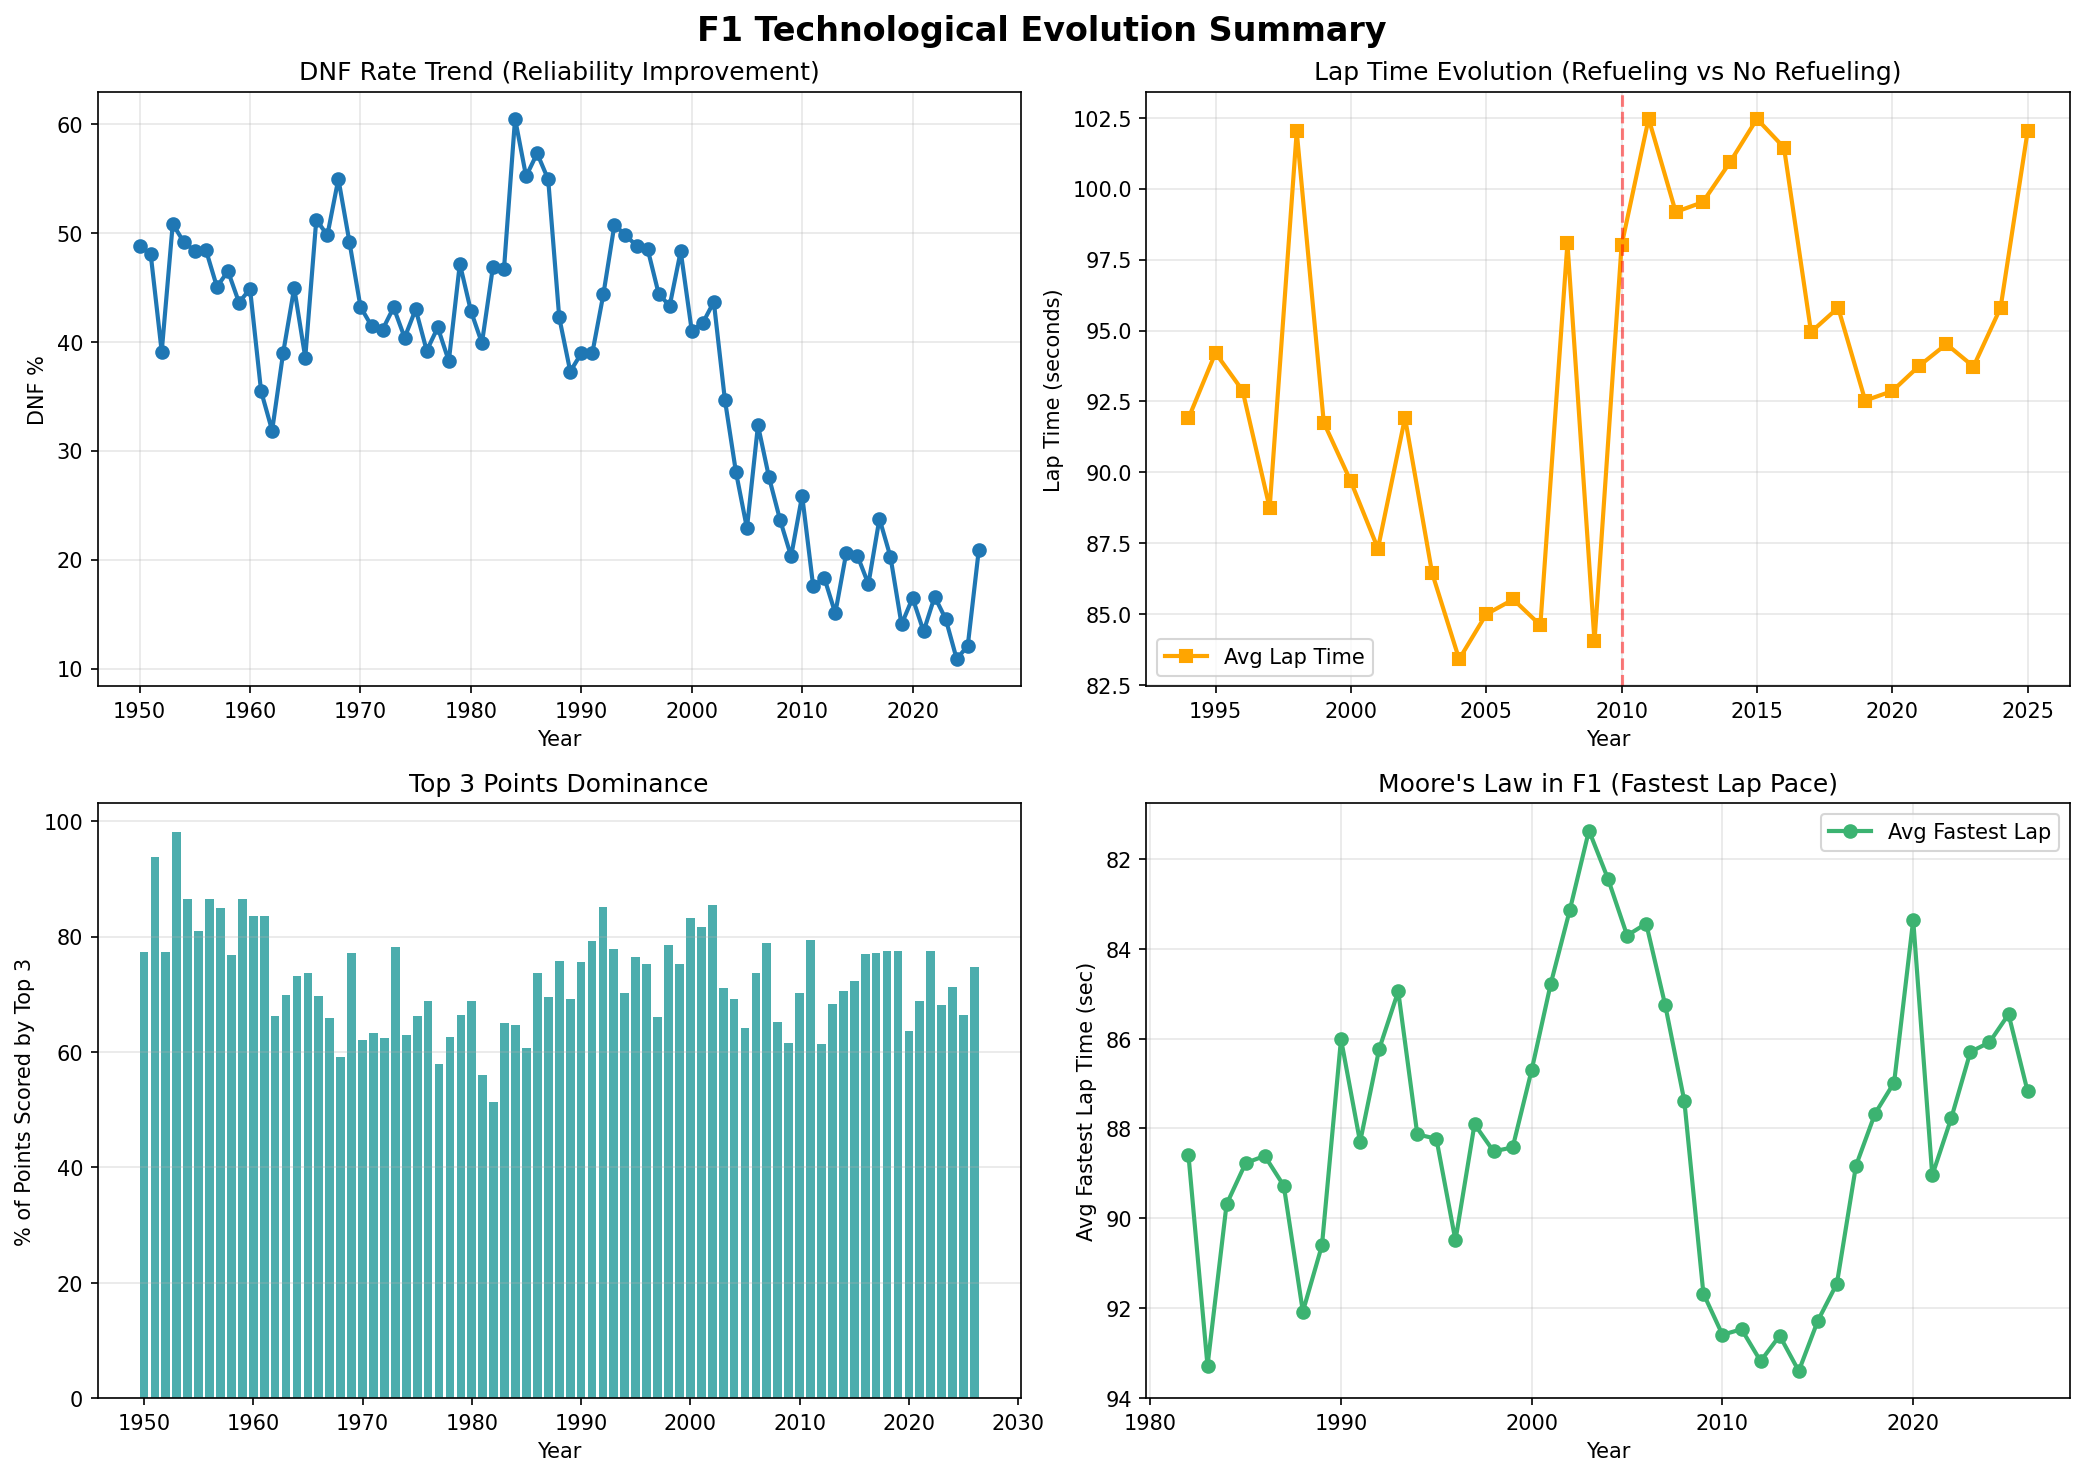
\includegraphics[keepaspectratio]{pres/F1Pandas/images/f1_analysis_summary.png}}
  \caption{Panel zbiorczy}
\end{figure}

\begin{center}\rule{0.5\linewidth}{0.5pt}
\end{center}

\subsection{4. Podsumowanie i wnioski}\label{podsumowanie-i-wnioski}

Czego nauczyły nas dane:

\begin{enumerate}
    \def\labelenumi{\arabic{enumi}.}
  \item
    \textbf{Auta są dużo bardziej niezawodne niż kiedyś.} Odsetek aut, które nie kończą wyścigu, spadł
    3--4 razy od lat 60. To najwyraźniejszy dowód postępu technicznego.
  \item
    \textbf{Pełny bak realnie spowalnia auto.} Widać to na różnych torach i w różnych latach --- a zakaz
    tankowania z 2010 roku jest dobrze widoczny w danych.
  \item
    \textbf{Dominacja zespołów chodzi w cyklach.} Czasem walka jest wyrównana, czasem rządzi jeden zespół.
    Teraz dominacja znów rośnie.
  \item
    \textbf{Auta nie jeżdżą szybciej co roku.} Nowe przepisy dwa razy (2009 i 2014) cofnęły rozwój. Postęp
    nie jest równy.
  \item
    \textbf{Niektóre „rankingi talentu'' potrafią mylić.} Trzeba uważać, jak liczy się dane wskaźniki ---
    bo łatwo wyciągnąć z nich błędny wniosek.
\end{enumerate}

\subsubsection{Ograniczenia i co dalej}\label{ograniczenia-i-co-dalej}

\begin{itemize}
    \tightlist
  \item
    Miara „punkty na sezon'' faworyzuje nowsze zespoły --- można ją poprawić, licząc punkty sprawiedliwiej
    w obrębie każdego sezonu albo patrząc na liczbę tytułów.
  \item
    Analiza najszybszych okrążeń miesza tory o różnej długości --- można to poprawić, uwzględniając
    długość toru.
  \item
    Projekt tylko \textbf{opisuje} przeszłość. Następny krok to \textbf{przewidywanie sezonu 2026} --- czyli model
    uczenia maszynowego (np. Random Forest), który na podstawie lat ze zmianą przepisów (2014, 2022)
    spróbuje zgadnąć, jak zmieni się układ sił. Dane są już przygotowane, ale model jeszcze nie powstał.
\end{itemize}

\begin{center}\rule{0.5\linewidth}{0.5pt}
\end{center}

\subsection{5. Załączniki}\label{zaux142ux105czniki}

\begin{longtable}[c]{@{}
    >{\raggedright\arraybackslash}p{(\linewidth - 4\tabcolsep) * \real{0.20}}
    >{\raggedright\arraybackslash}p{(\linewidth - 4\tabcolsep) * \real{0.38}}
  >{\raggedright\arraybackslash}p{(\linewidth - 4\tabcolsep) * \real{0.43}}@{}}
  \toprule\noalign{}
  Załącznik & Gdzie & Co to \\
  \midrule\noalign{}
  \endhead
  \bottomrule\noalign{}
  \endlastfoot
  \textbf{Kod źródłowy (notebook)} & \href{Project1.ipynb}{\texttt{Project1.ipynb}} & Cały kod: wczytanie danych → pytania SQL → analiza → wykresy \\
  \textbf{Baza danych} & \texttt{f1.db} & Lokalna baza DuckDB z danymi F1 (1950--2026) \\
  \textbf{Lista zależności} & \href{pyproject.toml}{\texttt{pyproject.toml}} & Spis bibliotek potrzebnych do uruchomienia \\
  \textbf{Prezentacja (slajdy)} & \href{pres/F1Pandas/slides.md}{\texttt{pres/F1Pandas/slides.md}} & Prezentacja w formacie Slidev (Markdown) \\
  \textbf{Prezentacja (PDF)} & \href{pres/F1Pandas/slides-export.pdf}{\texttt{pres/F1Pandas/slides-export.pdf}} & Prezentacja jako PDF \\
  \textbf{Prezentacja (PPTX)} & \href{pres/F1Pandas/slides-export.pptx}{\texttt{pres/F1Pandas/slides-export.pptx}} & Prezentacja jako PowerPoint \\
  \textbf{Wykresy} & \texttt{pres/F1Pandas/images/} & Gotowe obrazki (PNG) \\
\end{longtable}

\subsubsection{Użyte narzędzia}\label{uux17cyte-narzux119dzia}

\begin{itemize}
    \tightlist
  \item
    \textbf{Język:} Python (wersja 3.13 lub nowsza)
  \item
    \textbf{Baza danych:} DuckDB (pytania w języku SQL)
  \item
    \textbf{Liczenie na danych:} pandas, numpy
  \item
    \textbf{Wykresy:} matplotlib, seaborn
  \item
    \textbf{Pobieranie danych:} kagglehub (zbiór F1 z Kaggle)
  \item
    \textbf{Prezentacja:} Slidev
\end{itemize}

\subsubsection{Jak uruchomić}\label{jak-uruchomiux107}

\begin{Shaded}
  \begin{Highlighting}[]
    \ExtensionTok{uv}\NormalTok{ sync                       }\CommentTok{\# zainstaluj potrzebne biblioteki}
    \ExtensionTok{uv}\NormalTok{ run jupyter notebook       }\CommentTok{\# otwórz notebook Project1.ipynb}
  \end{Highlighting}
\end{Shaded}

\end{document}
